\section{Pruebas}
Para comprobar el funcionamiento de los programas se usaron los siguientes archivos wav.\\
Para realizar el filtrado mediante el producto en frecuencia, se uso como entrada para el programa de la transformada discreta de Fourier el siguiente archivo:
\begin{figure}[H]
	\centering
	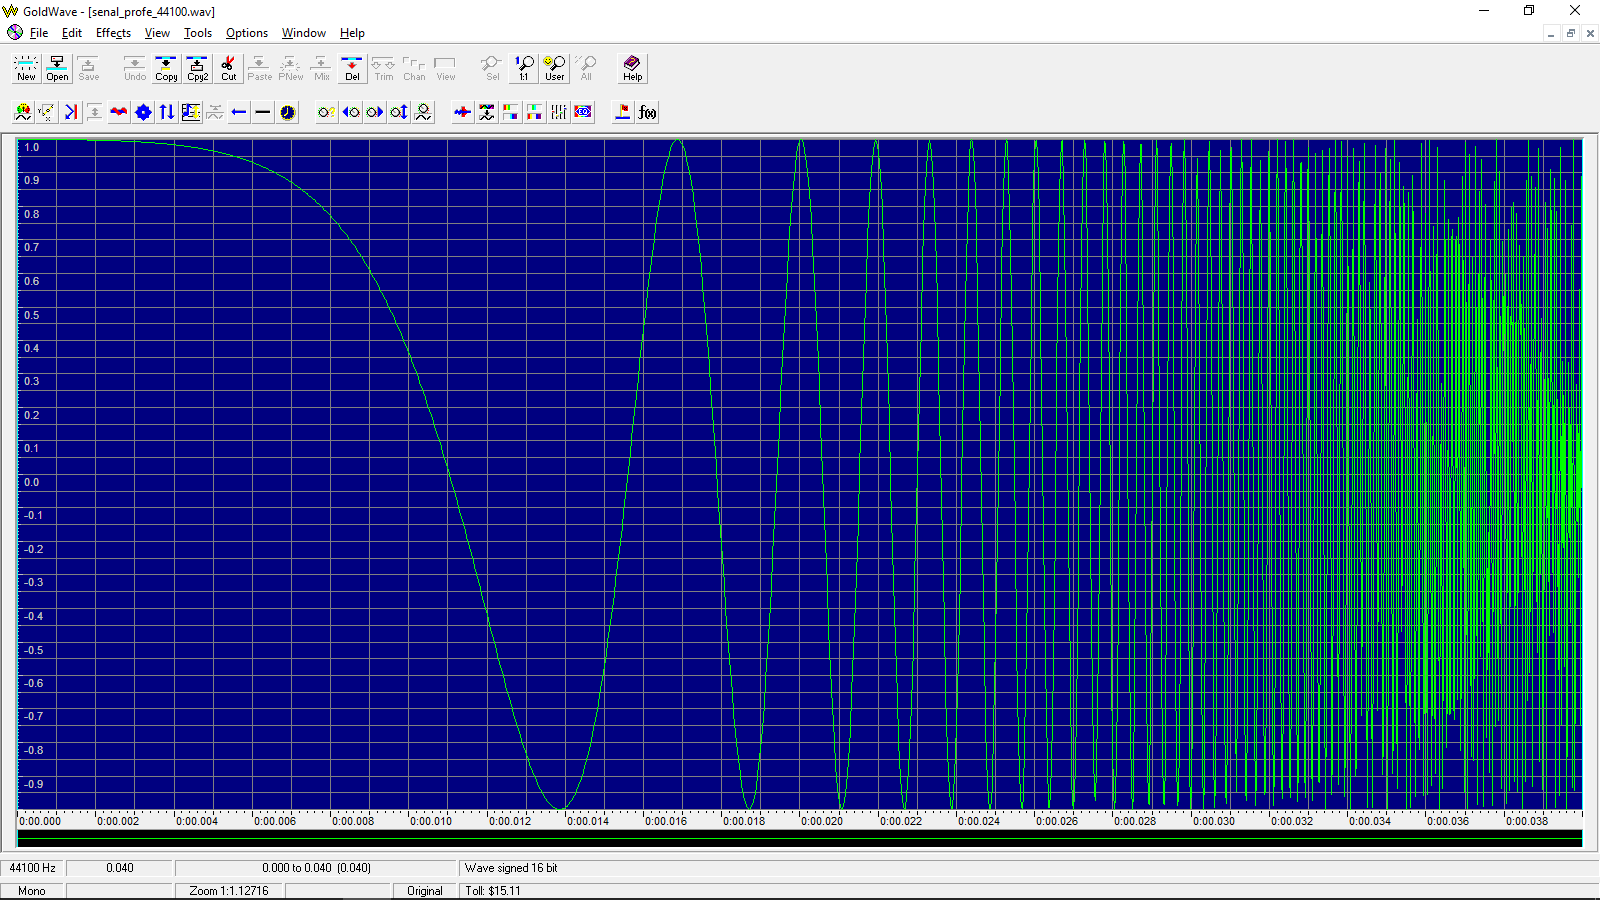
\includegraphics[scale=.35]{img/entrada.png}
	\caption{Entrada para TDF}
	\label{fig:prueba1}		
\end{figure}
El cual tiene una frecuencia de muestreo de 44100 muestras/s y una duración de .04 segundos.\\ A diferencia del archivo usado en el reporte 02A-Simulación circuito RC, donde la duración del archivo era de 1 segundo, para esta prueba se disminuyo la duración para que el número de muestras que tuviera que procesar el programa de la TDF no fuera tan grande (con esa duración y frecuencia de muestreo el total de muestras fue de 1764) y no demorara mucho tiempo ejecutándose. La función usada en el archivo fue: cos(2*pi*t*(exp(log(20)+n/N*6.6))).\newpage
La salida obtenida del programa TDF fue la siguiente:
\begin{figure}[H]
	\centering
	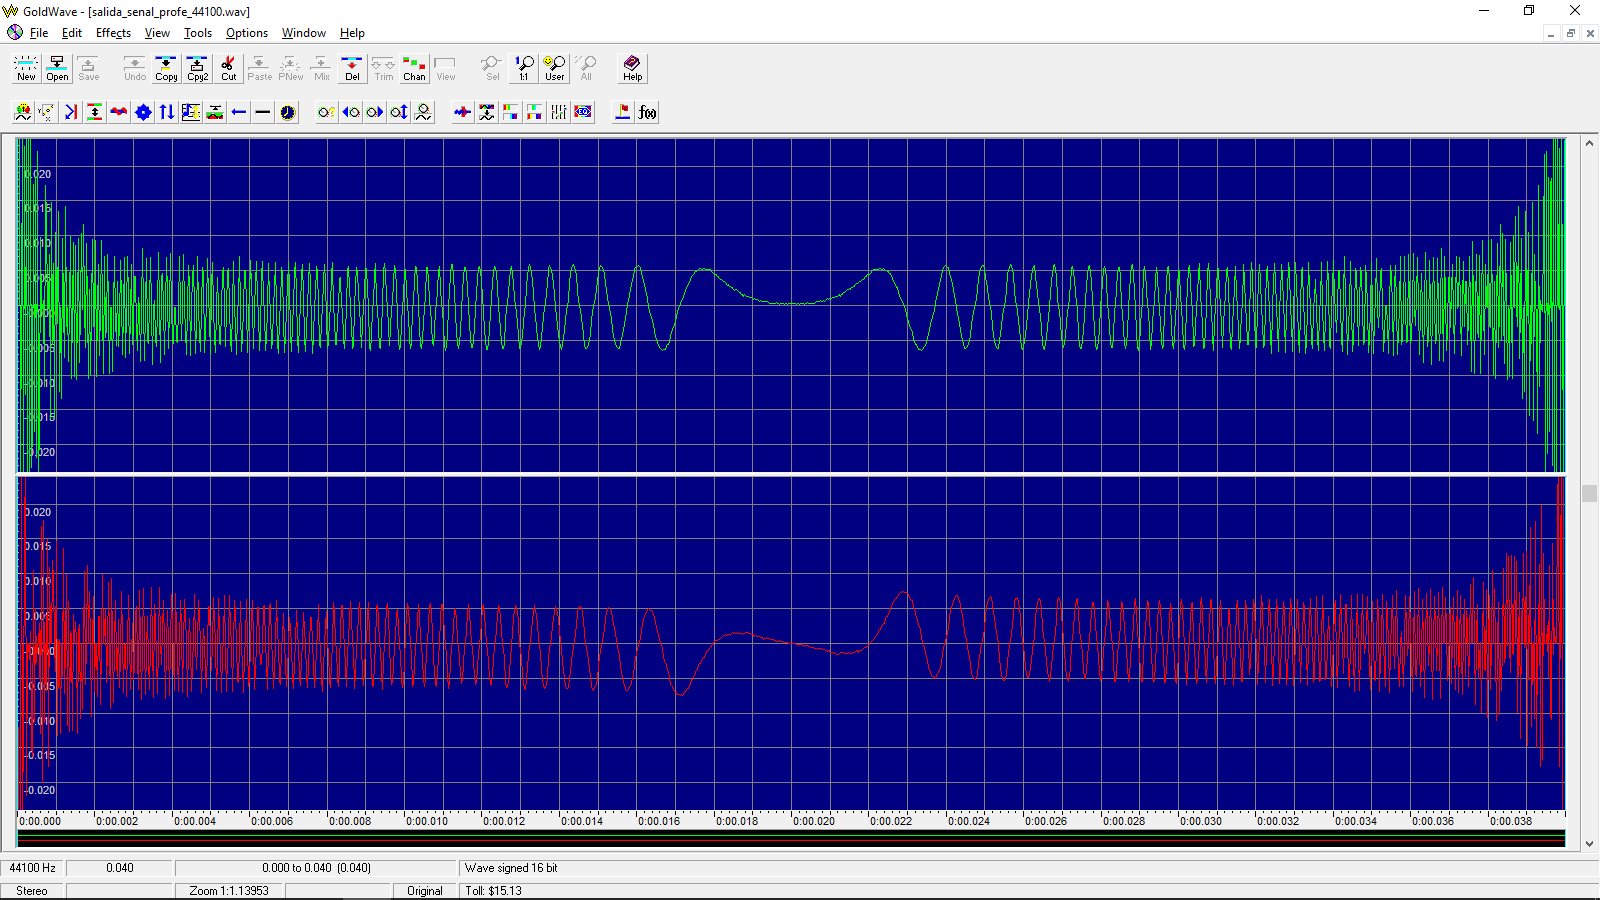
\includegraphics[scale=.3]{img/salidaTDF.png}
	\caption{Salida TDF}
	\label{fig:prueba2}		
\end{figure}
El filtro para realizar el producto se muestra en la siguiente Figura, cabe señalar que se modelo un filtro ideal con una frecuencia de corte de 1000Hz. Se creo, seleccionando solamente el canal izquierdo del archivo e ingresando la siguiente función:(step(n)-step(n-40))+step(n-(1764-40)).
\begin{figure}[H]
	\centering
	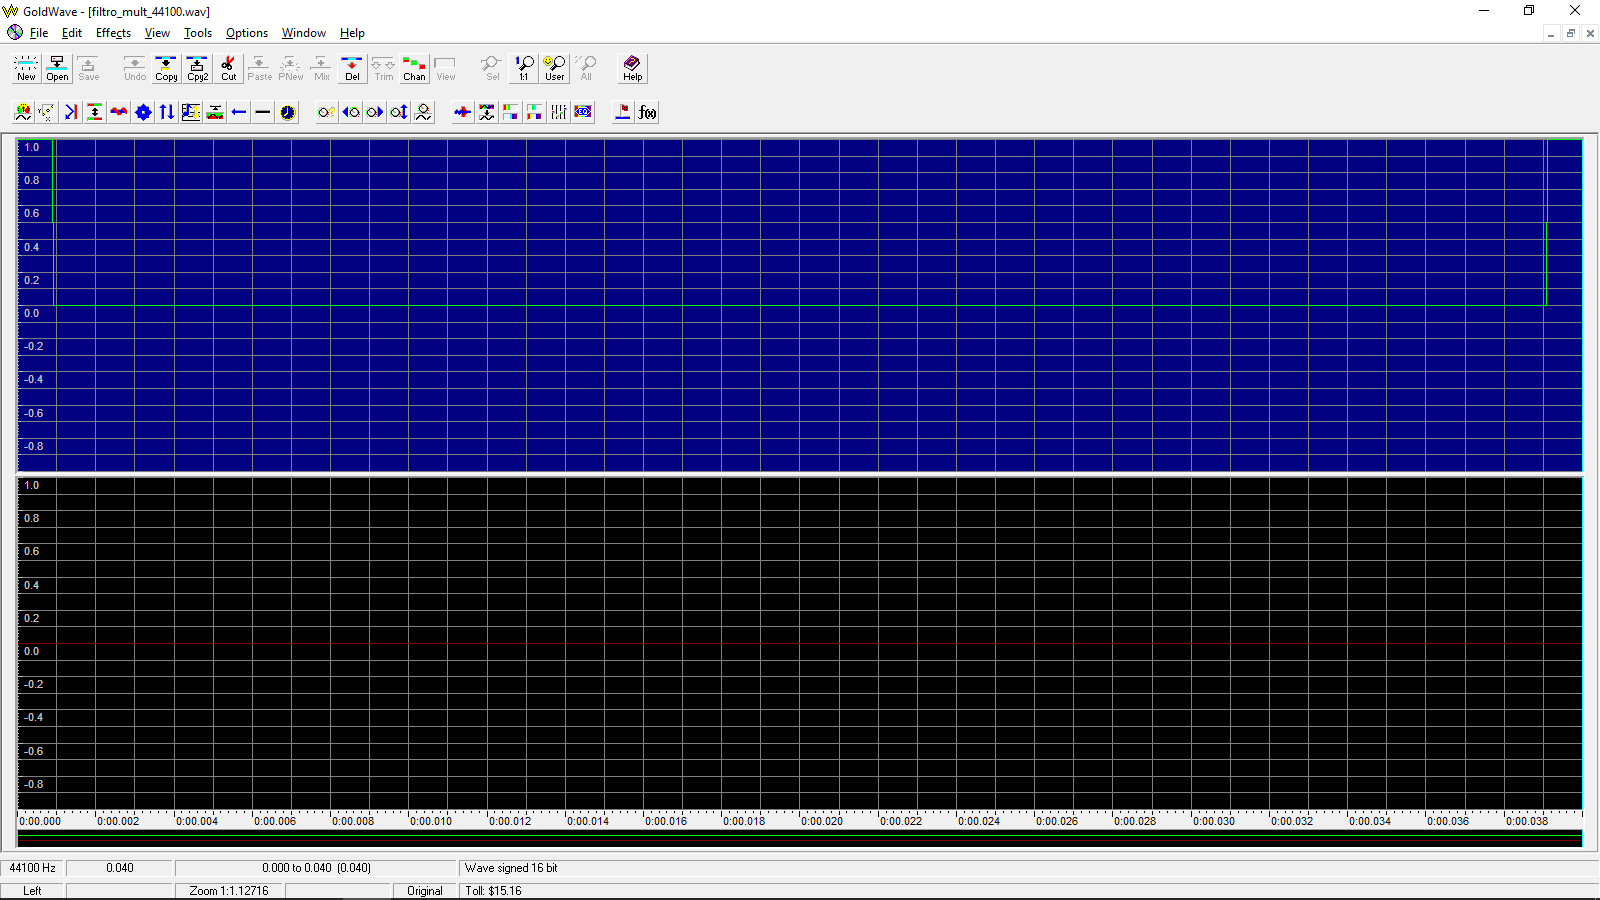
\includegraphics[scale=.3]{img/filtro.png}
	\caption{Filtro ideal con una frecuencia de corte de 1000Hz}
	\label{fig:prueba3}		
\end{figure}
Posteriormente, la salida obtenida de la TDF y el filtro fueron multiplicados usando el programa producto.exe, y se obtuvo la siguiente salida:
\begin{figure}[H]
	\centering
	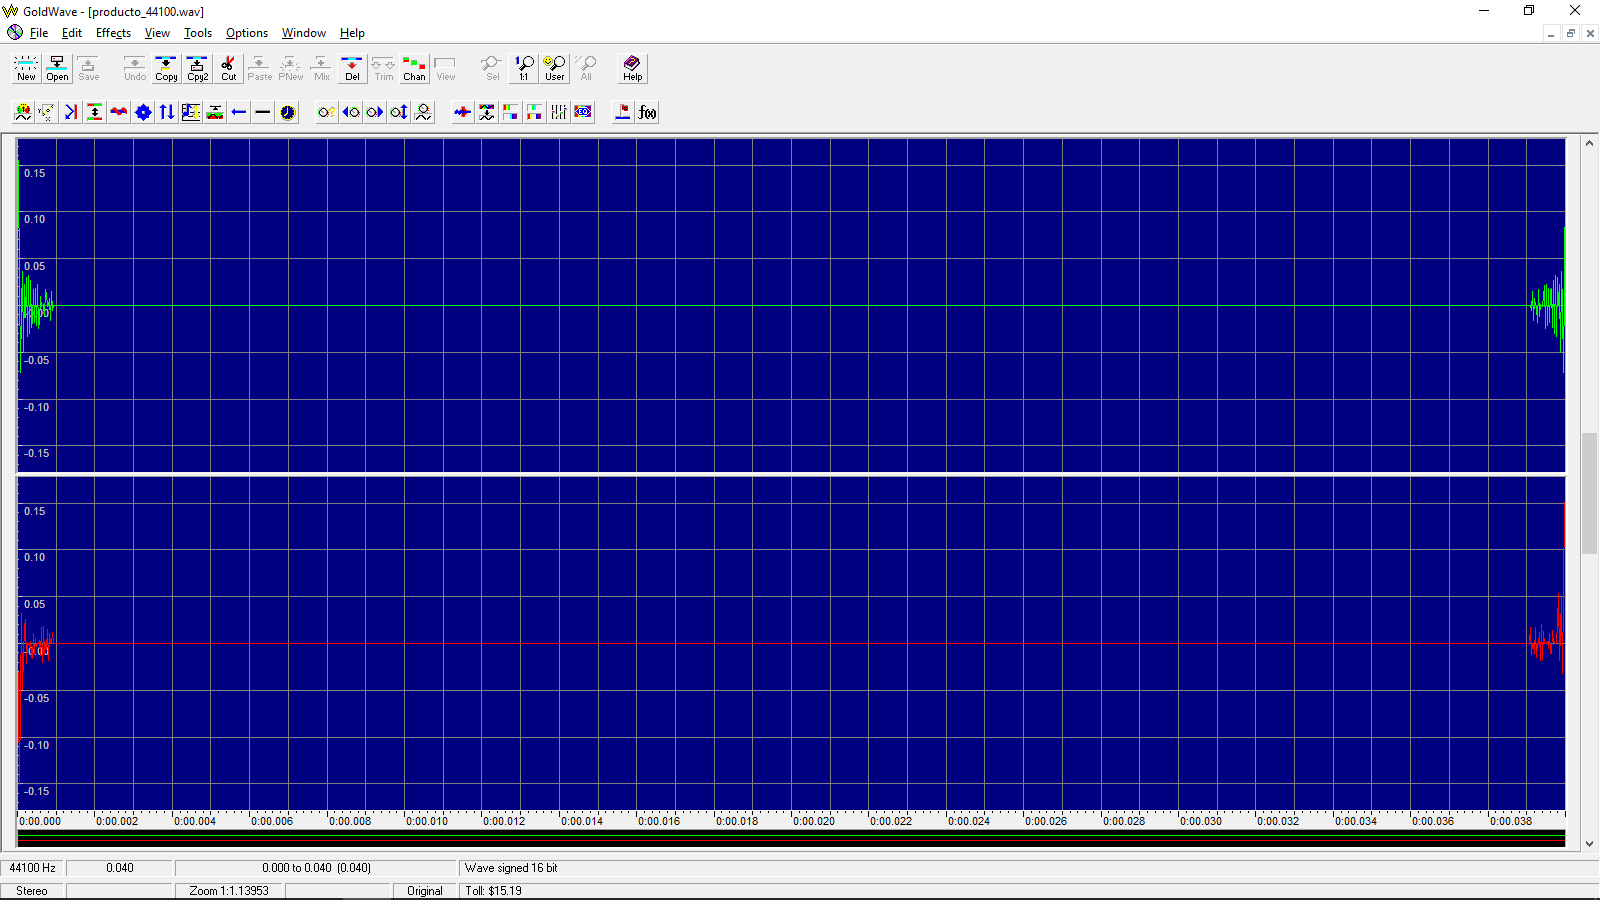
\includegraphics[scale=.35]{img/producto.png}
	\caption{Producto obtenido de multiplicar la salida de la TDF y el filtro ideal}
	\label{fig:prueba4}		
\end{figure}
A la salida obtenida por el programa del producto, finalmente fue ingresado al programa que calcula TDF Inversa, y se obtuvo la siguiente salida.
\begin{figure}[H]
	\centering
	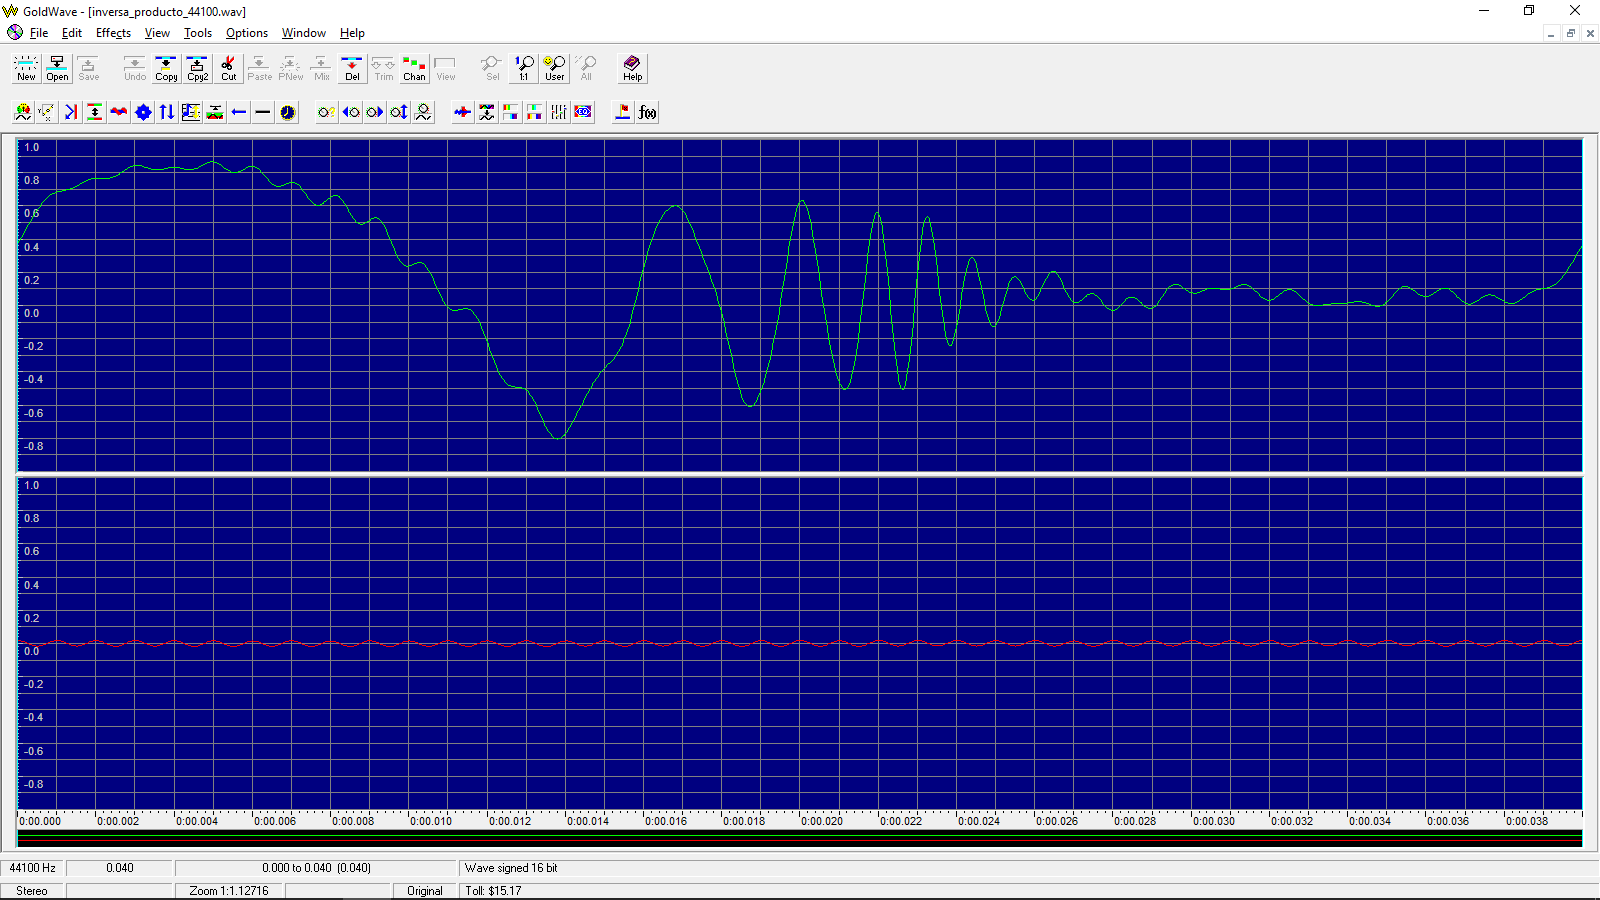
\includegraphics[scale=.32]{img/salida.png}
	\caption{Salida obtenida de la TDFI}
	\label{fig:prueba5}		
\end{figure}
Para comprobar que el resultado fuera el correcto, a la señal original de entrada se le filtro usando Goldwave, de lo cual se obtuvo la siguiente salida:
\begin{figure}[H]
	\centering
	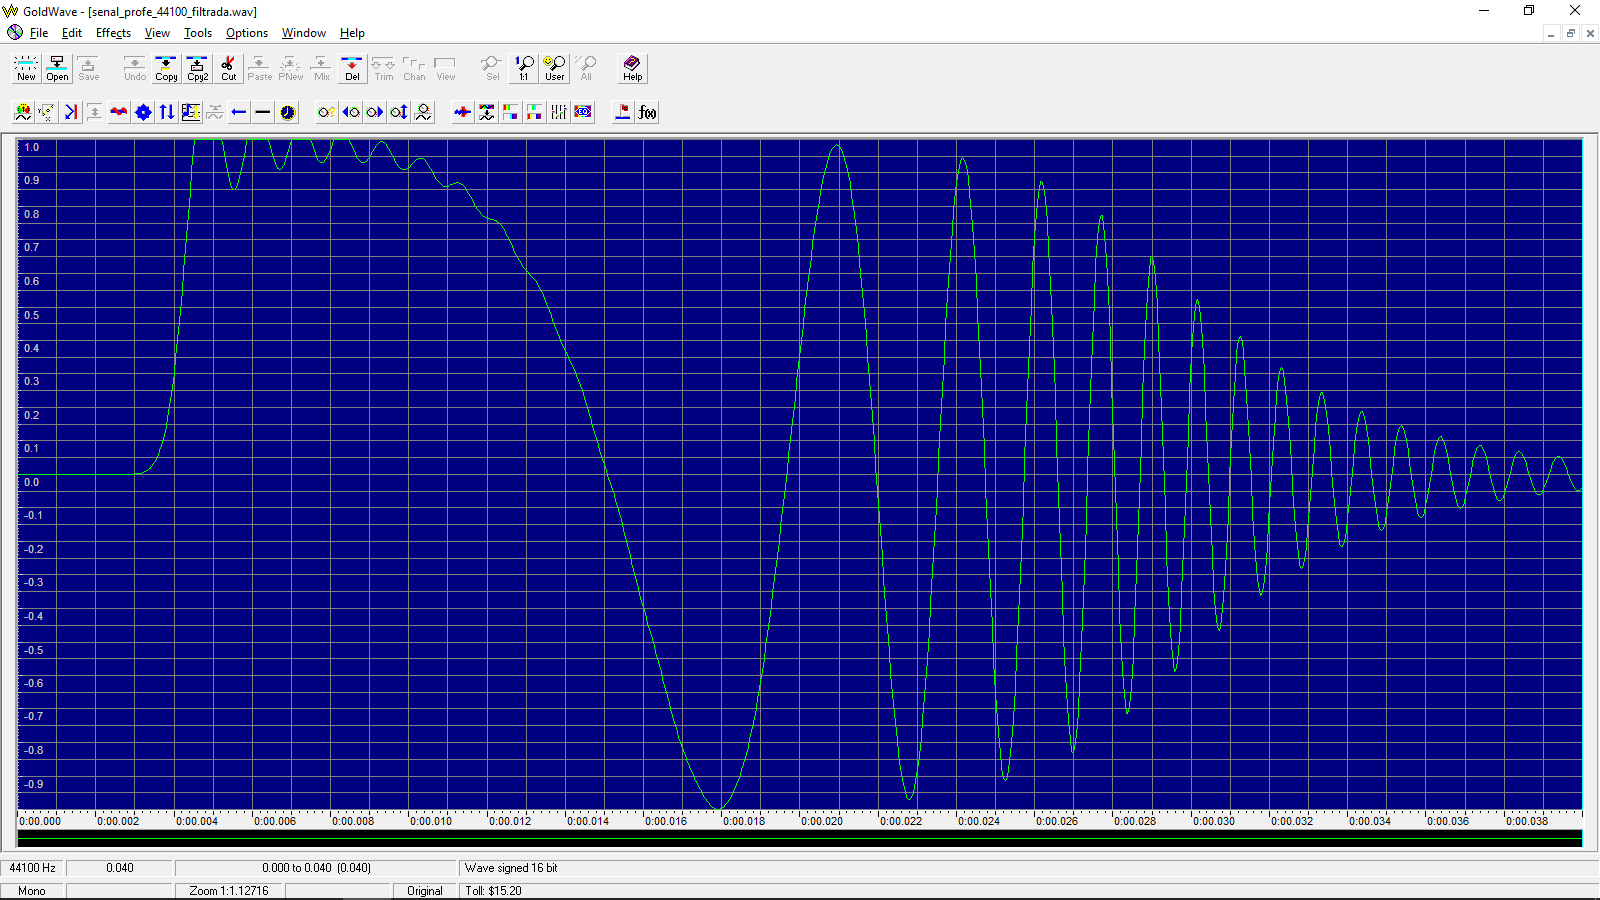
\includegraphics[scale=.32]{img/salida_goldwave.png}
	\caption{Señal original filtrada usando Goldwave}
	\label{fig:prueba6}		
\end{figure}
Como se puede observar, el filtrado realizado mediante frecuencia no es tan preciso como el hecho por Goldwave pero tiene una gran similitud con este mismo. En trabajo posterior, se repite este proceso pero usando la Transformada Rápida de Fourier (FFT).